%
% CSE Electronic Homework Template
% Last modified 8/23/2018 by Jeremy Buhler

\documentclass[11pt]{article}
\usepackage[left=0.7in,right=0.7in,top=1in,bottom=0.7in]{geometry}
\usepackage{fancyhdr} % for header
\usepackage{graphicx} % for figures
\usepackage{amsmath}  % for extended math markup
\usepackage{amssymb}
\usepackage[bookmarks=false]{hyperref} % for URL embedding
\usepackage[noend]{algpseudocode} % for pseudocode
\usepackage[plain]{algorithm} % float environment for algorithms

%%%%%%%%%%%%%%%%%%%%%%%%%%%%%%%%%%%%%%%%%%%%%%%%%%%%%%%%%%%%%%%%%%%%%%
% STUDENT: modify the following fields to reflect your
% name/ID, the current homework, and the current problem number

% Example: 
%\newcommand{\StudentName}{Jeremy Buhler}
%\newcommand{\StudentID{123456}

\newcommand{\StudentName}{Dingyu Wang (Howard)}
\newcommand{\StudentID}{COMP 642: Machine Learning}
\newcommand{\HomeworkNumber}{3}

%%%%%%%%%%%%%%%%%%%%%%%%%%%%%%%%%%%%%%%%%%%%%%%%%%%%%%%%%%%%%%%%%%%%%%%%
% You can pretty much leave the stuff up to the next line of %%'s alone.

% create header and footer for every page
\pagestyle{fancy}
\fancyhf{}
\lhead{\textbf{\StudentName}}
\chead{\textbf{\StudentID}}
\rhead{\textbf{HW \HomeworkNumber}}
\cfoot{\thepage}

% preferred pseudocode style
\algrenewcommand{\algorithmicprocedure}{}
\algrenewcommand{\algorithmicthen}{}

% ``do { ... } while (cond)''
\algdef{SE}[DOWHILE]{Do}{doWhile}{\algorithmicdo}[1]{\algorithmicwhile\ #1}%

% ``for (x in y ... z)''
\newcommand{\ForRange}[3]{\For{#1 \textbf{in} #2 \ \ldots \ #3}}

% these are common math formatting commands that aren't defined by default
\newcommand{\union}{\cup}
\newcommand{\isect}{\cap}
\newcommand{\ceil}[1]{\ensuremath \left\lceil #1 \right\rceil}
\newcommand{\floor}[1]{\ensuremath \left\lfloor #1 \right\rfloor}

%%%%%%%%%%%%%%%%%%%%%%%%%%%%%%%%%%%%%%%%%%%%%%%%%%%%%%%%%%%%%%%%%%%%%%
\usepackage[utf8]{inputenc}
\usepackage[english]{babel}
\setlength{\parindent}{0em}
\setlength{\parskip}{1em}
 \usepackage{pythonhighlight}
\usepackage{graphicx}
\graphicspath{ {./images/} }


\begin{document}

% STUDENT: Your text goes here!
1) \\
a)
\\
\\
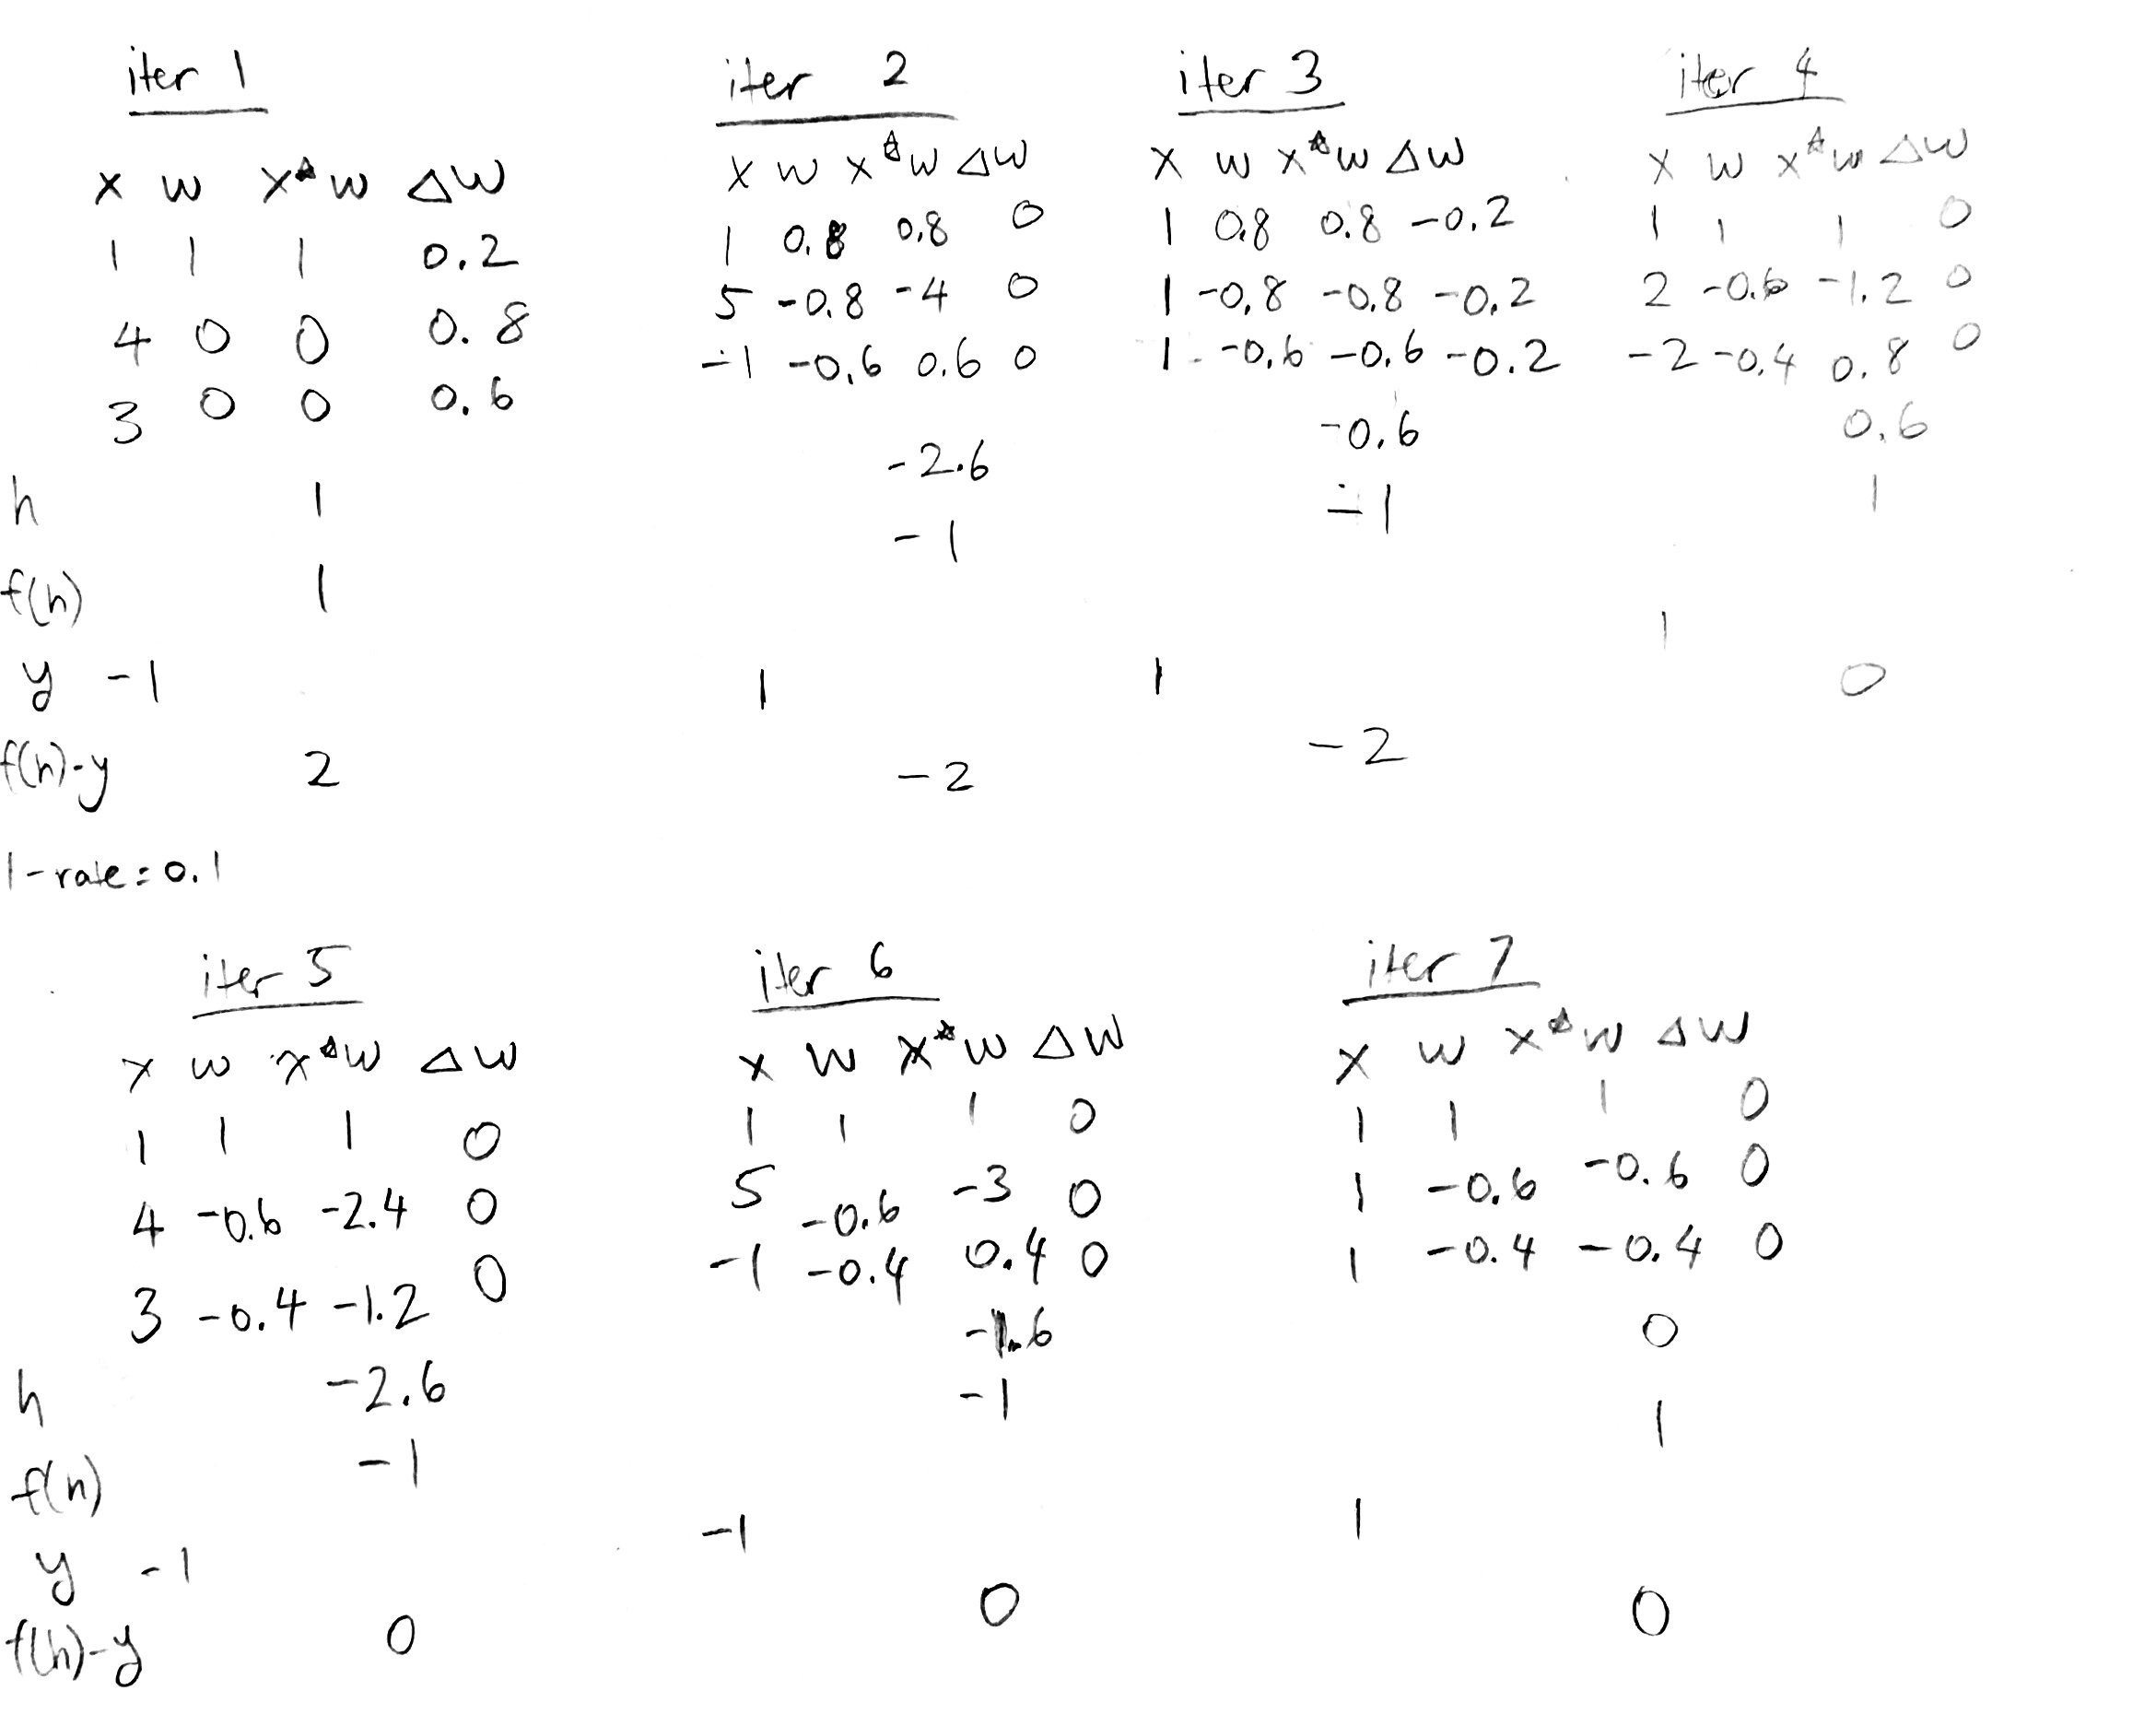
\includegraphics[scale=0.15]{hand1}
\\
\\
b) \\
No, a single perceptron cannot solve the problem. The dataset is not linearly separable, which you can clearly see from plotting it. After 10 iterations, the does not converge. Perceptron learning algorithm can solve problems where the data set is linearly separable. It cannot solve problems where more complex boundaries are required. \\
\\
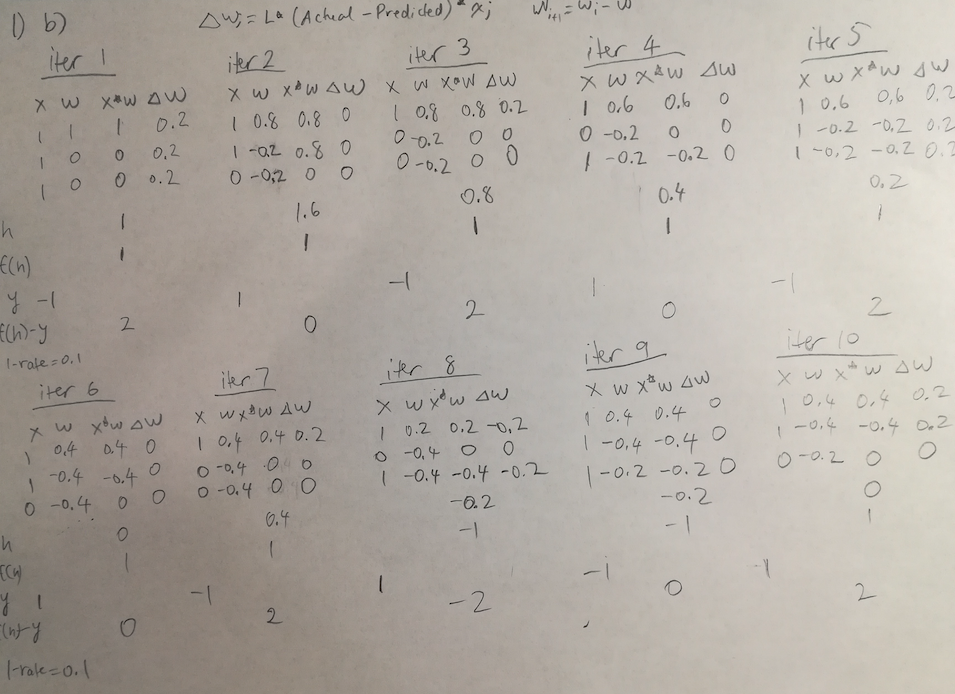
\includegraphics[scale=0.35]{perceptronhand}
\\

c) \\
Here is the perceptron code we have to fill in. \\
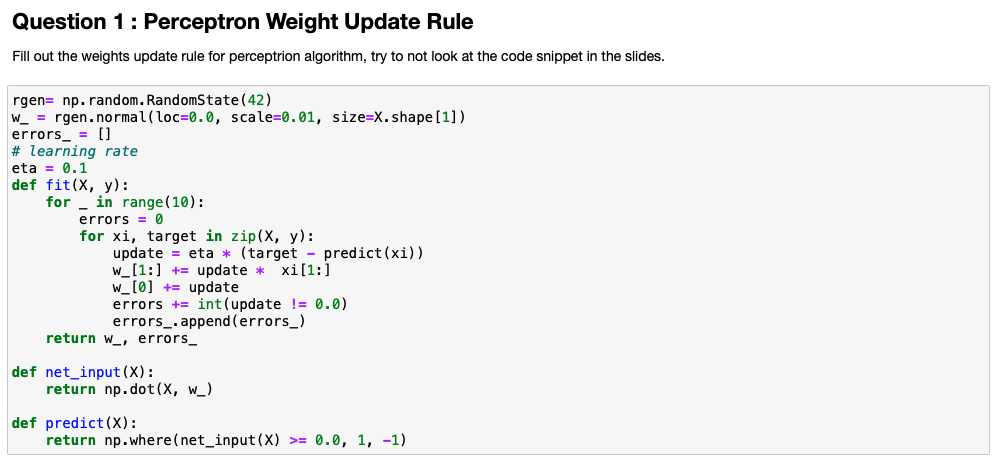
\includegraphics[scale=0.4]{perceptron}
\\
\\
2) \\
\\
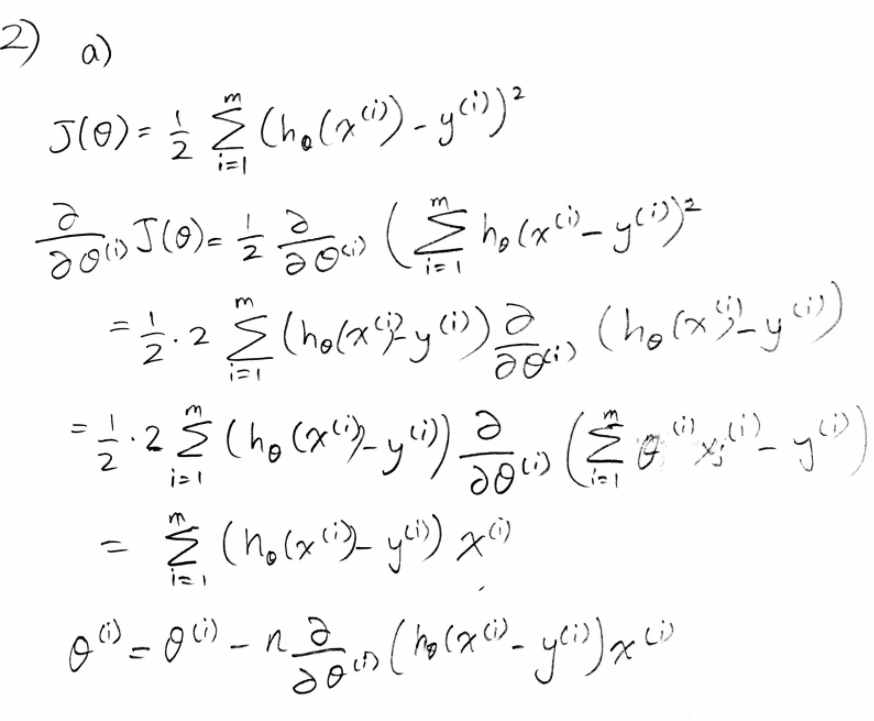
\includegraphics[scale=0.32]{adaline}

b) \\
Here is the adaline code we have to fill in. \\
\\
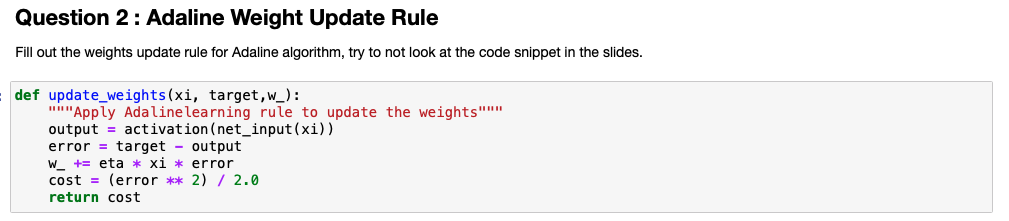
\includegraphics[scale=0.4]{adalinecode}
\\
\\
3) \\
a) 
Here is the logistic regression code we have to fill in. \\
\\
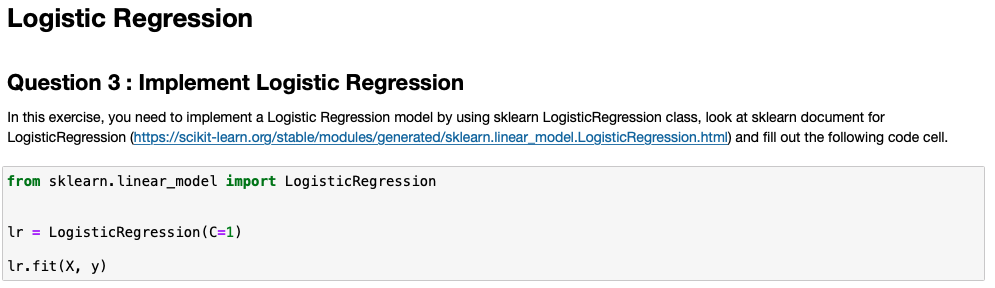
\includegraphics[scale=0.4]{logistic}
\\
\\
b) \\
I think the best is to include all 4 features: sepal\_length, sepal\_width, petal\_length, petal\_width. That uses all the information we have, and 4 features is not that many.
\\
\\
4) \\
For the perceptron algorithm, the decision boundary was closer to the red (-1). For the adaline algorithm, the decision boundary was closer to the blue (+1). The separating line had a positive slope. The decision boundary for logistic regression had a negative slope unlike the other two. It was also slightly closer (depending on the C value) to the middle way point between the two closest -1 and +1 points.

\end{document}
